\begin{table}[]
    \centering
    \footnotesize
    \caption[Characterization of some popular embedding operations.]{Characterization of the embedding operations in \Cref{sec:characterization-and-implications}. The compute-per-lookup ratio captures code complexity. The memory footprint defines storage requirements for all embedding vectors. The temporal locality proxies cache efficiency through the Cumulative Distribution Function ($CDF$) of the vector reuse distance. The spatial locality proxies prefetcher efficiency through the number of embedding elements in each vector.}
    \resizebox{\columnwidth}{!}{%
    \begin{tabular}{clccccc}
        \toprule
            \makecell[c]{\textbf{Op}} & 
            \makecell[l]{\textbf{Loop hierarchy}} & 
            $\frac{\textbf{N}_\textbf{compute}}{\textbf{N}_\textbf{lookups}}$ &
            \makecell[c]{\textbf{Memory} \\ \textbf{footprint}} &
            \makecell[c]{\textbf{Temporal locality} \\ \textbf{(reuse distance CDF)}} &
            \makecell[c]{\textbf{Spatial locality} \\ \textbf{(vector dim.)}}\\
        \toprule
            \makecell[c]{SpMM \\(GNNs)} &% \\ (\Cref{sec:characterization-and-implications-graph-learning})} &
            \makecell[l]{$\forall$ vertex in graph\\
                        \hspace{0.5em}$\forall$ neighbor of vertex\\
                            \hspace{1em}\textbf{lookup} vector\\
                            \hspace{1em}\textbf{rescale} vector\\
                            \hspace{1em}\textbf{accumulate} vector} &
            \normalsize$\frac{2}{1}$ &
            \makecell{GBs} &
            \vcentered{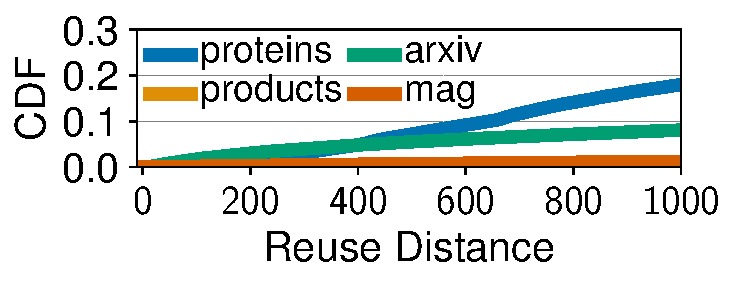
\includegraphics[width=.3\linewidth]{img_cdf_gnn.pdf}} &
            8-349\\ 
        \hline
            \makecell[c]{MP} &% \\ (\Cref{sec:characterization-and-implications-graph-learning})} &
            \makecell[l]{$\forall$ vertex in graph\\
                        \hspace{0.5em}\textbf{lookup} vertex vector\\
                        \hspace{0.5em}$\forall$ neighbor of vertex\\
                            \hspace{1em}\textbf{lookup} neighbor vector\\
                            \hspace{1em}\textbf{multiply} vert-neigh vecs\\
                            \hspace{1em}\textbf{scale} and \textbf{accumulate} vec\\
                        \hspace{0.5em}\textbf{multiply-accumulate} vec} &
            \normalsize$\leq\frac{5}{2}$ &
            \makecell{GBs} &
            \vcentered{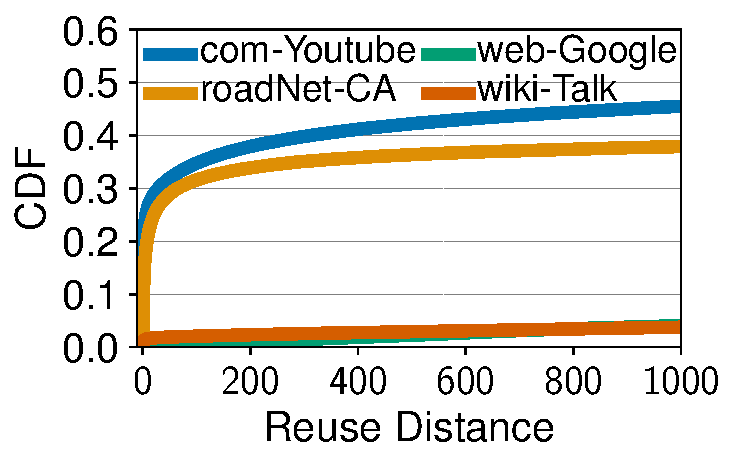
\includegraphics[width=.3\linewidth]{img_cdf_mp.pdf}} &
            128\\
        \hline
            \makecell[c]{KGs} &% \\ (\Cref{sec:characterization-and-implications-graph-learning})} &
            \makecell[l]{$\forall$ sample in batch\\
                            \hspace{0.5em}\textbf{lookup} vector\\
                            \hspace{0.5em}\textbf{compute} h-r-l norm} &
            \normalsize$\frac{4}{3}$ &
            \makecell{GBs} &
            \vcentered{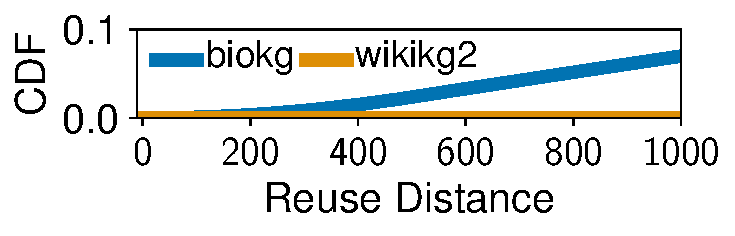
\includegraphics[width=.3\linewidth]{img_cdf_kg.pdf}} &
            512\\
        \hline
            \makecell[c]{EB \\ (DLRMs)} &% \\ (\Cref{sec:characterization-and-implications-dlrms})} &
            \makecell[l]{$\forall$ segment in batch\\
                            \hspace{0.5em}$\forall$ category in segment\\
                                \hspace{1.0em}\textbf{lookup} vector\\
                                \hspace{1.0em}\textbf{accumulate} vector} &
            \normalsize$\frac{1}{1}$ &
            \makecell{TBs} &
            \vcentered{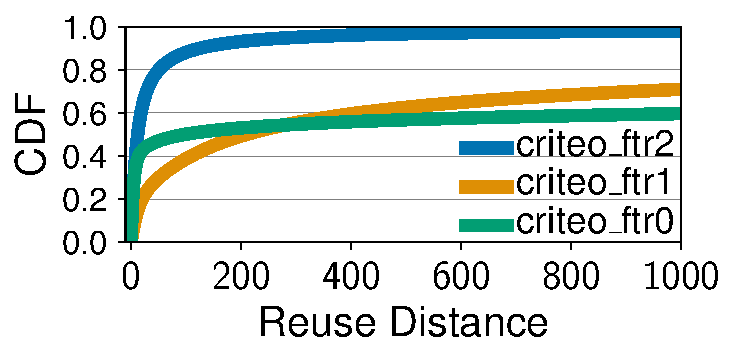
\includegraphics[width=.3\linewidth]{img_cdf_dlrm.pdf}} &
            32-256\\
        \hline
            \makecell[c]{SpAttn \\ (LLMs)} &% \\ (\Cref{sec:characterization-and-implications-llms})} &
            \makecell[l]{$\forall$ block in Q input\\
                        \hspace{0.5em}$\forall$ block in K input\\
                            \hspace{1.0em}$\forall$ token in K block\\
                                \hspace{1.5em}\textbf{lookup} K vector\\
                                \hspace{1.5em}$\forall$ token in Q block\\
                                    \hspace{2em}\textbf{copy} K vector} &
            \normalsize$0$ &
            \makecell{MBs-GBs} &
            \vcentered{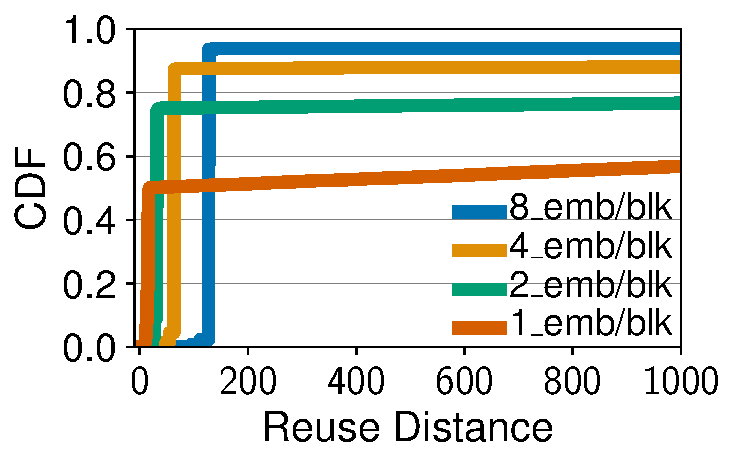
\includegraphics[width=.3\linewidth]{img_cdf_llm.pdf}} &
            $\leq$ 8x8x512\\
        \bottomrule
    \end{tabular}
    }
    \label{tab:characterization}
    %\vspace{-2em}
\end{table}

        
        
        
        
        